\documentclass{beamer}


\usepackage{amsmath}
\usepackage[style=alphabetic,url=true]{biblatex}
\usepackage{environ}
\usepackage{geometry}
\usepackage{graphicx}
\usepackage{tikz}
\usepackage[T2A]{fontenc}
\usepackage[utf8]{inputenc}
\usepackage[cache=false]{minted}
\usepackage{amsmath}
\usepackage{amsfonts}
\usepackage{amssymb}
\usepackage{calrsfs}
\usepackage{animate}
\usepackage{xmpmulti}


% \usetheme{Bergen}

\usecolortheme{beaver}

\setbeamertemplate{itemize item}[circle]
\setbeamertemplate{itemize subitem}{--}
\addtobeamertemplate{navigation symbols}{}{
  \usebeamerfont{footline}%
  \usebeamercolor[fg]{footline}%
  \hspace{1em}%
  \insertframenumber/\inserttotalframenumber
}
\graphicspath{ {./graphics/} }
\definecolor{code-background}{gray}{0.85}
\setminted[Python]{fontsize=\tiny}
\BeforeBeginEnvironment{minted}{\medskip}
\AfterEndEnvironment{minted}{\medskip}
\usetikzlibrary{matrix}
\tikzset{
  stack/.style={
    matrix of nodes,
    nodes={
      fill=lightgray,draw,text=black,font=\sffamily\bfseries,
      text height=11pt,text depth=3pt,baseline=center, minimum width=1cm
    },
    column sep=-\pgflinewidth/2
  }
}

\title{
  Біткоїн та криптовалютні технології \\
  Лекція 8: Біткоїн-гаманці
}

\author{Юрій Жикін}
\date{27 березня, 2025}

\begin{document}

\frame{\titlepage}

\begin{frame}
  \frametitle{Набір UTXO}
  \begin{itemize}
  \item Увесь біткоїн в обігу представлений у вигляді \textbf{набору UTXO} -
    набору всіх невикористаних транзакційних виходів.
  \item Кожна ``монета'' (\textbf{UTXO}) складається з певної кількості
    \textbf{сатоші} та відповідного скрипту замикання.
  \item Щоб перевірити отриману транзакцію, користувач має переконатися, що
    транзакція правильно сформована, і що виходи, які вона використовує, входять
    до \textbf{множини UTXO}.
  \item Весь протокол Bitcoin працює для забезпечення \textbf{узгодженості}
    \textbf{набору UTXO}.
  \end{itemize}
\end{frame}

\begin{frame}
  \frametitle{Володіння біткоїном}
  \begin{itemize}
  \item \textbf{Володіння біткоїном} означає, що користувач може надати
    правильний \textbf{скрипт відмикання} до \textbf{скрипту замикання} деяких
    виходів з \textbf{набору UTXO}.
  \item Скрипти блокування є відкритими, тому кожен невикористаний транзакційний
    вихід повинен мати унікальний скрипт блокування.
  \item Інакше можна легко обчислити, скільки біткоїнів належить певній певному.
  \item \textbf{Біткоїн-гаманець} - це зазвичай програмне забезпечення для
    зберігання даних, необхідних для створення скриптів відмикання до
    відповідних UTXO.
  \end{itemize}
\end{frame}

\begin{frame}
  \frametitle{Стандартні скрипти замикання}
  \begin{itemize}
  \item \textbf{P2PK} — Pay to Public Key
    \break
    \begin{tabular}{rl}
      &\tiny\mintinline[bgcolor=code-background]{Lisp}{<pubKey> OP_CHECKSIG;} \\
    \end{tabular}
  \item \textbf{P2MS} — Pay to Multi-Signature
    \break
    \begin{tabular}{rl}
      &\tiny\mintinline[bgcolor=code-background]{Lisp}{<M> <pk1> ... <pkN> <N> OP_CHECKMULTISIG;} \\
    \end{tabular}
  \item \textbf{P2PKH} — Pay to Public Key Hash
    \break
    \begin{tabular}{rl}
      &\tiny\mintinline[bgcolor=code-background]{Lisp}{OP_DUP OP_HASH160 <pubKeyHash> OP_EQUALVERIFY OP_CHECKSIG;} \\
    \end{tabular}
  \item \textbf{P2SH} — Pay to Script Hash
    \break
    \begin{tabular}{rl}
      &\tiny\mintinline[bgcolor=code-background]{Lisp}{OP_HASH160 <scriptHash> OP_EQUAL;} \\
    \end{tabular}
  \item \textbf{P2WPKH} — Pay to \textbf{Witness} Public Key Hash
    \break
    \begin{tabular}{rl}
      &\tiny\mintinline[bgcolor=code-background]{Lisp}{OP_0 <20-byte-witness-data>;} \\
    \end{tabular}
  \item \textbf{P2WSH} — Pay to \textbf{Witness} Script Hash
    \break
    \begin{tabular}{rl}
      &\tiny\mintinline[bgcolor=code-background]{Lisp}{OP_0 <32-byte-witness-data>;} \\
    \end{tabular}
  \end{itemize}
\end{frame}

\begin{frame}
  \frametitle{Відокремлений свідок}
  \begin{itemize}
  \item Софтфорк у мережі, активований 24 серпня 2017 року.
  \item Запропонований у серії \textbf{пропозицій щодо покращення Біткоїна}
    (Bitcoin Improvement Proposals) — BIP-0141, BIP-0143, BIP-0144 та BIP-0148.
  \item Основна ідея полягає у винесенні великих скриптів відмикання з даних
    транзакцій, що включаються в блоки.
  \end{itemize}
\end{frame}

\begin{frame}
  \frametitle{Біткоїн-адреси 1/4}
  \begin{itemize}
  \item Біткоїн використовує кілька орієнтованих на людей способів кодування
    адрес та ключів:
    \begin{itemize}
    \item \textbf{Base58Check} \break
      \begin{tabular}{rl}
        &${\scriptstyle \mathit{Base58Check}(t, data) = \mathit{Base58}(t + data + \mathit{HASH256}(t + data)[0:4])}$ \\
      \end{tabular}
      \break
      де \textit{Base58} використовує алфавіт
      \break
      \begin{tabular}{rl}
        &${\scriptstyle 123456789ABCDEFGHJKLMNPQRSTUVWXYZabcdefghijkmnopqrstuvwxyz}$ \\
      \end{tabular}
    \item \textbf{Bech32}
      \break
      \begin{tabular}{rl}
        &${\scriptstyle \mathit{Bech32}(t, data) = t + "1" + \mathit{Base32'}(data + \mathit{Bech32Checksum}(t, data))}$ \\
      \end{tabular}
      \break
      де \textit{Base32'} використовує алфавіт
      \break
      \begin{tabular}{rl}
        &${\scriptstyle qpzry9x8gf2tvdw0s3jn54khce6mua7l}$ \\
      \end{tabular}
    \end{itemize}
  \end{itemize}
\end{frame}

\begin{frame}
  \frametitle{Біткоїн-адреси 2/4}
  \begin{itemize}
  \item Формати адрес для \textbf{P2PK} та \textbf{P2MS} не визначені.
  \item Формат адреси для \textbf{P2PKH}
    \break
    \begin{tabular}{rl}
      &\tiny\mintinline[bgcolor=code-background]{Lisp}{OP_DUP OP_HASH160 <pubKeyHash>
        OP_EQUALVERIFY OP_CHECKSIG;} \\
      &${\scriptstyle A_{\mathit{p2pkh}} = \mathit{Base58Check}(0x00 +
        pubKeyHash)}$ \\
      &{\scriptsize \quad\quad\quad \textbf{1}7VZNX1SN5NtKa8UQFxwQbFeFc3iqRYhem} \\
      &${\scriptstyle A'_{\mathit{p2pkh}} = \mathit{Base58Check}(0x6F +
        pubKeyHash)}$ \\
      &{\scriptsize \quad\quad\quad \textbf{m}ipcBbFg9gMiCh81Kj8tqqdgoZub1ZJRfn} \\
    \end{tabular}
  \end{itemize}
\end{frame}

\begin{frame}
  \frametitle{Біткоїн-адреси 3/4}
  \begin{itemize}
  \item Формат адреси для \textbf{P2SH}
    \break
    \begin{tabular}{rl}
      &\tiny\mintinline[bgcolor=code-background]{Lisp}{OP_HASH160 <scriptHash> OP_EQUAL;} \\
      &${\scriptstyle A_{\mathit{p2sh}} = \mathit{Base58Check}(0x05 +
        scriptHash)}$ \\
      &{\scriptsize \quad\quad\quad \textbf{3}EktnHQD7RiAE6uzMj2ZifT9YgRrkSgzQX} \\
      &${\scriptstyle A'_{\mathit{p2sh}} = \mathit{Base58Check}(0xC4 +
        scriptHash)}$ \\
      &{\scriptsize \quad\quad\quad \textbf{2}MzQwSSnBHWHqSAqtTVQ6v47XtaisrJa1Vc} \\
    \end{tabular}
  \end{itemize}
\end{frame}

\begin{frame}
  \frametitle{Біткоїн-адреси 4/4}
  \begin{itemize}
  \item Формат адреси для \textbf{P2WPKH/P2WSH}
    \break
    \begin{tabular}{rl}
      &\tiny\mintinline[bgcolor=code-background]{Lisp}{OP_0 <20-or-32-byte witnessData>;} \\
      &${\scriptstyle A_{\mathit{p2wpkh/p2wsh}} = \mathit{Bech32}("bc" +
        witnessVersion + witnessData)}$ \\
      &{\scriptsize \quad\quad\quad \textbf{bc1}qw508d6qejxtdg4y5r3zarvary0c5xw7k\textbf{v8f3t4}} \\
      &${\scriptstyle A'_{\mathit{p2wpkh/p2wsh}} = \mathit{Bech32}("tb" +
        witnessVersion + witnessData)}$ \\
      &{\scriptsize \quad\quad\quad \textbf{tb1}qw508d6qejxtdg4y5r3zarvary0c5xw7k\textbf{xpjzsx}} \\
    \end{tabular}
  \end{itemize}
\end{frame}

\begin{frame}
  \frametitle{Зберігання криптографічних ключів 1/2}
  \begin{itemize}
  \item Усі стандартні скрипти замикання/відмикання базуються на наданні
    підпису, який відповідає публічному ключу, до якого прив'язаний скрипт
    блокування.
  \item Оскільки форма скрипту стандартизована, \textit{єдиним елементом, що
      відрізняється}, є \textbf{публічний ключ або його хеш}.
  \item Єдиним елементом даних, необхідними для створення стандартного скрипту
    відмикання до стандартного скрипту замикання, є \textit{відповідний
      приватний ключ}.
  \end{itemize}
\end{frame}

\begin{frame}
  \frametitle{Зберігання криптографічних ключів 2/2}
  \begin{itemize}
  \item Усі сучасні Біткоїн-гаманці є \textbf{сховищами криптографічних ключів}
    з додатковою функціональністю:
    \begin{itemize}
    \item безпечне зберігання приватних ключів для ``монет'', що належать
      користувачу,
    \item генерація нових приватних і публічних ключів та адрес,
    \item для кожного нового блоку або транзакції — перевірка, чи відповідає її
      скрипт блокування стандартному скрипту блокування/розблокування, який
      підходить до одного з наявних ключів (необов'язково),
    \item конструювання нових транзакцій шляхом вибору підмножини UTXO для
      знищення та створення нових UTXO з додавання відповідних скриптів
      розблокування (необов'язково).
    \end{itemize}
  \end{itemize}
\end{frame}

\begin{frame}
  \frametitle{Прості гаманці з пулом ключів}
  \begin{itemize}
  \item Найпростішим Біткоїн-гаманцем є \textbf{один приватний ключ}.
  \item Адреса є видимою в ланцюгу, тому при \textbf{повторному використанні
      адрес} легко обчислити кількість біткоїнів, що належать одному й тому ж
    користувачу.
  \item \textit{Повторне використання адрес} — це погана практика, тому
    необхідна генерація нового ключа для кожної вхідної транзакції.
  \item Гаманець — це файл, який містить список ключів для всіх ``монет'', що
    належать користувачу.
  \item Після кожної отриманої транзакції необхідно створювати нову резервну
    копію.
  \item Розмір сховища ключів постійно зростає, а видаляти старі ключі
    небезпечно, оскільки неможливо гарантувати, що їхні адреси не будуть
    використані повторно.
  \end{itemize}
\end{frame}

\begin{frame}[fragile]
  \frametitle{Ієрархічні детерміністичні гаманці 1/2}
  \begin{itemize}
  \item \textbf{Ієрархічні детерміністичні гаманці} (\textbf{HD-гаманці}) були
    вперше запропоновані у 2011 році та стандартизовані у BIP-0032 у 2012 році.
  \item Основна ідея — використання \textbf{кореневого приватного ключа}, з
    якого генеруються дерево приватних ключів.
  \item \textbf{Приватний ключ у ієрархії може бути використаний для генерації
      дочірніх приватних ключів}.
    \begin{tabular}{rl}
      &${\scriptstyle \mathit{CKD_{priv}}(k_{par}, c_{par}, i) = \mathit{HMACSHA512}(c_{par},
        k_{par}G||i) = I}$ \\
      &${\scriptstyle k_i = I[0:32] + k_{par} \pmod{n}}$ \\
      &${\scriptstyle c_i = I[32:64]}$ \\
    \end{tabular}
  \item \textbf{Публічний ключ у ієрархії може бути використаний для генерації
      дочірніх публічних ключів, але не їхніх приватних ключів}.
    \begin{tabular}{rl}
      &${\scriptstyle \mathit{CKD_{pub}}(K_{par}, c_{par}, i) = \mathit{HMACSHA512}(c_{par},
        K_{par}||i) = I}$ \\
      &${\scriptstyle K_i = (I[0:32])G + K_{par} = (I[0:32] + k_{par})G = k_iG}$ \\
      &${\scriptstyle c_i = I[32:64]}$ \\
    \end{tabular}
  \end{itemize}
\end{frame}

\begin{frame}[fragile]
  \frametitle{Ієрархічні детерміністичні гаманці 2/2}
  \begin{itemize}
  \item BIP-0039 визначає спосіб кодування кореневого ключа у вигляді
    послідовності слів.
  \item Більшість сучасних гаманців показують \textbf{BIP-0039-зерно}
    (\textbf{seed}) під час ініціалізації.
  \item Словник містить 2048 ($2^{11}$) слів.
  \item Послідовність з 12 слів містить 128 ($12 * 11 = 132$) криптографічної
    ентропії.
  \item Приклад:
\begin{minted}{text}
  fortune flush  weekend current
  key     hero   snake   leopard
  brisk   climb  timber  appear
\end{minted}
  \end{itemize}
\end{frame}

\begin{frame}
  \frametitle{Безпека: мобільні гаманці}
  \begin{itemize}
  \item Існують десятки застосунків-гаманців для мобільних пристроїв (iOS та
    Android):
    \begin{itemize}
    \item \textbf{BlueWallet} (iOS, Android, клієнт-сервер, можливість
      підключення до власного вузла),
    \item \textbf{BlockStream Green} (iOS, Android, клієнт-сервер),
    \item \textbf{Bitcoin Wallet} (Android, SPV-вузол).
    \end{itemize}
  \item Основний недолік — ключі зберігаються на пристрої, підключеному до
    мережі, що саме по собі погано з точки зору безпеки.
  \item Будь-яке порушення безпеки, яке дозволяє отримати доступ до даних на
    пристрої, може призвести до витоку ключів ключів.
  \item Підходить для повсякденних транзакцій із невеликими сумами біткоїнів.
  \end{itemize}
\end{frame}

\begin{frame}[fragile]
  \frametitle{Безпека: апаратні гаманці}
  \begin{minipage}{0.6\textwidth}\raggedright
    \begin{itemize}
    \item Апаратні гаманці — це спеціалізовані \textbf{ізольовані} пристрої,
      призначені для генерації та зберігання криптографічних ключів:
      \begin{itemize}
      \item \textbf{пристрої Trezor}
      \item \textbf{пристрої Ledger}
      \item \textbf{Coinkite Coldcard}
      \item \textbf{Blockstream Jade}
      \item \textbf{Shift Crypto BitBox02}
      \end{itemize}
    \end{itemize}
  \end{minipage}
  \begin{minipage}{0.3\textwidth}\raggedleft
    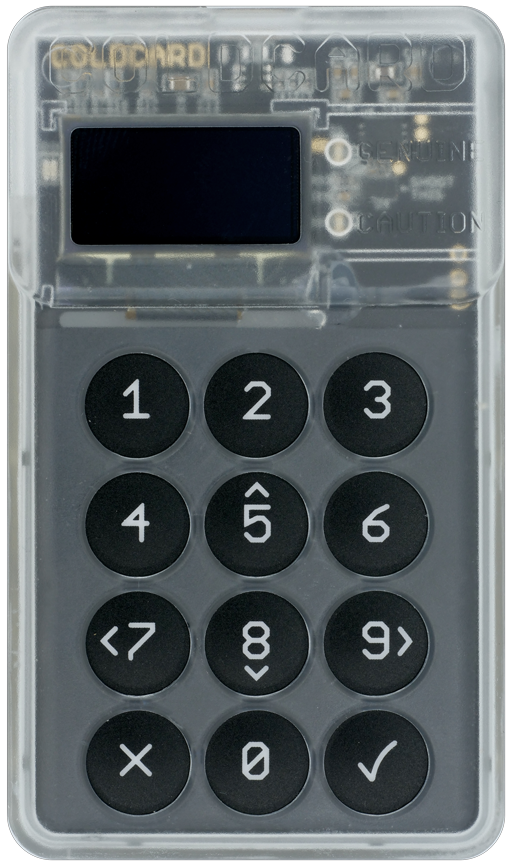
\includegraphics[width=0.7\linewidth]{coldcard-front}
  \end{minipage}
\end{frame}

\begin{frame}
  \frametitle{Безпека: холодне зберігання}
  \begin{itemize}
  \item \textbf{Холодне зберігання} — це будь-який метод зберігання, який не
    передбачає використання програмного забезпечення або електронних пристроїв.
  \item HD-зерно можна записати на аркуші паперу й зберігати у надійному місці,
    або навіть просто запам’ятати.
  \item Щоб скористатися біткоїнами з холодного сховища, потрібно спочатку
    перенести ключ на пристрій, що може підписувати транзакції (апаратний чи
    мобільний гаманець).
  \end{itemize}
\end{frame}

\begin{frame}
  \frametitle{Безпека: загальний підхід}
  \begin{itemize}
  \item \textbf{Достатньо безпечний підхід} до зберігання біткоїнів:
    \begin{itemize}
    \item згенерувати новий \textbf{кореневий приватний ключ} на
      спеціалізованому пристрої (апаратному гаманці),
    \item створити \textbf{холодну резервну копію} кореневого приватного ключа
      (паперовий гаманець або металевий пристрій для зберігання ключів),
    \item імпортувати \textbf{кореневий публічний ключ} на пристрій, який буде
      використовуватись для відстеження балансу (смартфон),
    \item \textbf{видалити приватний ключ із спеціалізованого пристрою}.
    \end{itemize}
  \end{itemize}
\end{frame}


\begin{frame}
  \frametitle{Кінець}
  \begin{center}
    Дякую за увагу!
  \end{center}
\end{frame}

\end{document}

%%% Local Variables:
%%% mode: latex
%%% TeX-master: t
%%% End:
